\documentclass{article}

\usepackage{amsmath}
\usepackage{amscd}
\usepackage{amssymb}
\usepackage{amsfonts}
\usepackage{amsthm}
\usepackage{amsfonts}
\usepackage{amsthm}

\usepackage{circuitikz}
\usepackage{pgf}
\usepackage{tikz}
\usetikzlibrary{arrows,snakes,backgrounds}
% \usetikz
\usepackage{subfig}

\usepackage[super]{nth}
% \usepackage{appendix}
% \usepackage{listings}
% \usepackage{color}

\usepackage{hyperref}
%\usepackage{url}

\usepackage{cleveref}

\usepackage{aviolov_style}
\usepackage{local_style}

\begin{document}


\title{The 2nd moment of the Hitting time of an OU Process} 
\author{Alexandre Iolov 
$<$\href{mailto:aiolo040@uottawa.ca}
		{aiolo040 at uottawa dot ca}$>$}

\date{\today}

\maketitle

\abstract{Calculate the 2nd moment of the hitting time of an OU process given
an arbitrary initial position}

\def \t {{ T}}

\section{Problem Formulation}
Given the following OU Model:
\begin{equation}
\begin{gathered}
dX_s = (\a - \frac{X_s}{\tc} ) \intd{s} + \b \intd{W_s},
\\
X(0) = x_0,
\\
\a > 0
\end{gathered}
\label{eq:X_evolution_uo}
\end{equation}
and a hitting time, $\t$, defined by
\begin{equation}
X_\t = \xth 
\quad \textrm{AND} \quad
X_{s < \t} < \xth
\end{equation}
we want an analytical expression for:
\begin{equation}
\Exp[\t^2|x_0]
\end{equation}
as a function of $\a,\tc,\b$

We can assume $\xth = 1.0$, but $x_0$ is arbitrary, that is - it is not
necessarily the 'equilibirum' value $.0$, indeed we will need to know
$\Exp[\t^2|x_0]$ for a whole range of $x_0$.

\subsection{Analytical Expressions for $\Exp[\t^2|x_0]$}

We will use the formulas/notation directly from \cite{Inoue1995}.
\begin{equation}
\Exp[\t^2] = \tc^2 \left[
2\phi_1^2(\eta) -
  \phi_2(\eta) -
  2\phi_1(\eta)\phi_1(\xi)+
  \phi_2(\xi)
  \right]
\end{equation}
where
\begin{eqnarray}
\xi &=& \boxed{(x_0 - \a\tc) \sqrt{\frac{2}{\b^2 \tc}}}
\\
\eta &=&
\boxed{(\xth -\a \tc )\sqrt{\frac{2}{\b^2 \tc}}}
\\
\phi_1(z)&=&
 \frac{1}{2} \sum_{n=1}^{\infty} \frac{(z \sqrt{2})^n}{n!}
 \Gamma\left(\tfrac{n}{2}\right)
\\
\phi_2(z)&=& 
 \frac{1}{2} \sum_{n=1}^{\infty} \frac{(z \sqrt{2})^n}{n!}
 \Gamma\left(\tfrac{n}{2}\right) \left( \psi\left(\tfrac{n}{2} \right) -
 \psi(1) \right)
\end{eqnarray}
where $\Gamma, \psi$ are the
\href{http://docs.scipy.org/doc/scipy/reference/generated/scipy.special.gamma.html#scipy.special.gamma}{Gamma}
and
\href{http://docs.scipy.org/doc/scipy/reference/generated/scipy.special.psi.html#scipy.special.psi}{digamma}
 functions respectively. Note that $\xth > x_0 \implies \eta > \xi$.

In the paper \cite{Inoue1995}, we are cautioned that evaluation of $\phi_k(z)$
directly is efficient and accurate as long as $z$ is positive and small. If $z$
is negative we will have an alternating series and a cancellation might cause
numerical errors. 

Actually, I cannot get this to work at all!!! 

% Instead we will use the Backward
% Kolmogorov equation, which is more useful since we need to calculate
% $\Exp[T^2|x_0]$ for a whole interval of $x_0$'s.

\subsection{Backward Kolmogorov equation}


Here we follow Jacobs, \cite{Jacobs}, in deriving and solving a differential
equation for $\Ttwo = \Exp[\t^2|x_0]$.

Basically we are calculating the mean-time-squared to exit an interval $[\xmin,
\xth]$. Theoretically, $\xmin = -\infty$, but for our purposes we will set it to
some finite value and impose reflecting boundaries there - this is a very good
approximation for $\xmin \ll 0$, as long as $\a>0$, which is what we have. 

Let $B(y,t|x) = \Prob[X_0 = y| X_t = x]$ for a fixed $x$. Then $B$ solves the
following (backward Kolmogorov) PDE:
\begin{equation}
-\di_t B = (\a - \frac y\tc)\di_yB - \frac {\b^2} 2 \di_y^2 B
\label{eq:backward_Xdensity}
\end{equation}

Let $\G(t,y)$ be the survival function for $T$ for $X_0 = y$. 
$$\G(t,y) = \Prob[T>t | X_0 = y] = \Prob[X_{s\leq t} \in [\xmin,
\xth] | X_0 = y]$$.

Because the dynamics do not depend explicitly on time, we have:
$$
\G(t,y) = \int_\xmin^\xth B(y,t|x) \intd{x}
$$
and so $\G$, being a definite integral of $B$ satisfies the same PDE:
\begin{equation}
-\di_t \G = (\a - \frac y\tc) \di_y\G - \frac {\b^2} 2 \di_y^2 \G
\label{eq:backward_SDF}
\end{equation}

With the BCs, ICs:
\begin{equation}
\begin{cases}
\G(t,\xth) = .0 & \quad (T = t \implies \Prob[T>t] = 0)
\\
\di_x \G(t,\xmin) = .0  & \quad (\textrm{due to reflecting boundary for X})
\\
\G(0, y) = 1. & \quad (T \textrm{ is definitely} > 0 \textrm{ for } x_0 \in
(\xmin, \xth) )
\end{cases}
\end{equation}

If we solve the PDE for $\G$ for $t \in [0,\infty)$, then we can calculate
$\Ttwo(x_0)$ as:
\begin{eqnarray}
\Ttwo(x_0) &=& \int_0^\infty t^2 \cdot (-\di_t\G(t,x_0)) \intd{t}
\\
		   &=& \int_0^\infty 2t \cdot \G(t,x_0) \intd{t}
\end{eqnarray}
assuming it exists.

Since $\Tone$ is an integral over time, we can reduce the PDE in
\cref{eq:backward_SDF} for the distribution to a BVP for the moment(s) by
integrating over time. Here is how this is done: multiply both sides  of
\cref{eq:backward_SDF} by $2t$, and integrate with respect to time:
\begin{equation}
\int_0^\infty 2t (-\di_t \G) \intd{t}
= 
\int_0^\infty  2t \left[ (\a - \frac y\tc) \di_y\G - \frac {\b^2} 2
\di_y^2 \G\right]
\intd{t}
\end{equation}
The LHS turns out to be $2\Tone$, so 
\begin{equation}
2\Tone
=(\a - \frac y\tc)   \di_y \Ttwo 
- \frac {\b^2} 2
\di_y^2 \Ttwo
\label{eq:BVP_Ttwo}
\end{equation}
Very similarly we can derive an equation for $\Tone$, namely:
\begin{equation}
1
=(\a - \frac y\tc)   \di_y \Tone 
- \frac {\b^2} 2
\di_y^2 \Tone
\label{eq:BVP_Tone}
\end{equation}
In both cases, the BCs will be:
\begin{equation}
\begin{cases}
\Ti(\xth) = .0 & \quad (\textrm{we are already spking})
\\
\di_x \Ti(\xmin) = .0  & \quad (\textrm{due to reflecting boundary for }X)
\end{cases}
\label{eq:BVP_Ti_BCs}
\end{equation}

\Cref{eq:BVP_Tone,eq:BVP_Ttwo} are seemingly 2nd order, but are actually
first order and can be written as:
\begin{equation}
f(y)
=U(y) S(y) 
- D S'(y) ; \quad  S(\xmin) = .0
\label{eq:BVP_T_generic}
\end{equation}
and we can recover $\Ti$ from $S$ via:
$$\Ti(x_0) =   -\int_{x_0}^\xth S(\xi)\intd{\xi}$$.
It is clear that thus defined, $\Ti$ will satisfy the BCs of
\cref{eq:BVP_Ti_BCs}.

Solving \cref{eq:BVP_T_generic} for $S$ gives:
\begin{eqnarray}
S(y) &=& - \exp\left(\smallint \tfrac UD \right) \cdot \int_\xmin^{y} 
\exp\left(-\int \tfrac UD\right) \frac{f(\xi)}D
\intd{\xi}
\\
 &=& - \exp\left( \frac{\a y - \frac{y^2}{2\tc}}D \right) 
 		\cdot 
 		\int_\xmin^{y}   \exp\left(- \frac{\a \xi - \tfrac{\xi^2}{2\tc}}D \right)
 		\frac{f(\xi)}D \intd{\xi}
\label{eq:BVP_T_generic_soln}
\end{eqnarray}

Actually, the analytical solution is not very useful for numerical calculations,
we are better off just calculating the numerical solutions to
\cref{eq:BVP_Tone,eq:BVP_Ttwo} directly.

Comparisons between simulations and the numerical solutions can be found in 
\begin{figure}[h]
\begin{center}
\subfloat[]
{
\label{fig:ab1}
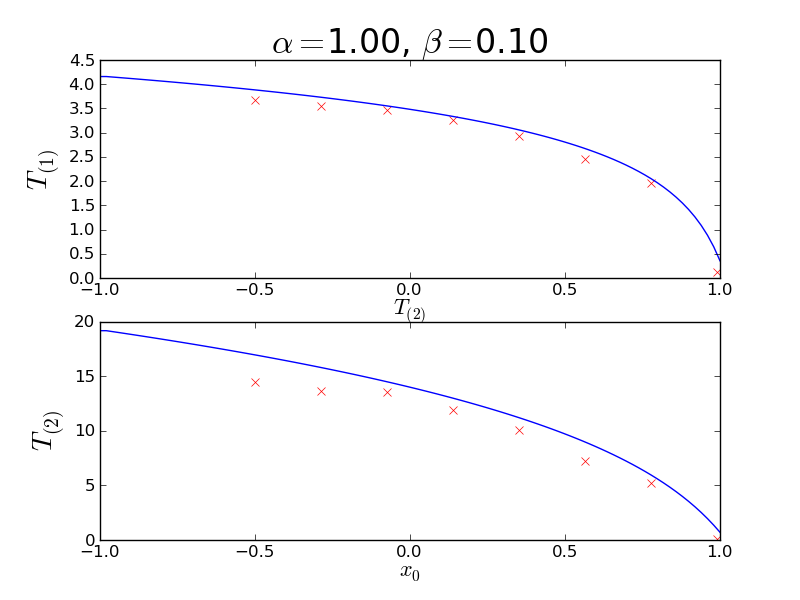
\includegraphics[width=0.48\textwidth]
{/home/alex/Workspaces/Latex/OptSpike/Figs/Moments_a=10_b=1_N=128.png}
}
\subfloat[ ]
{
\label{fig:ab2}
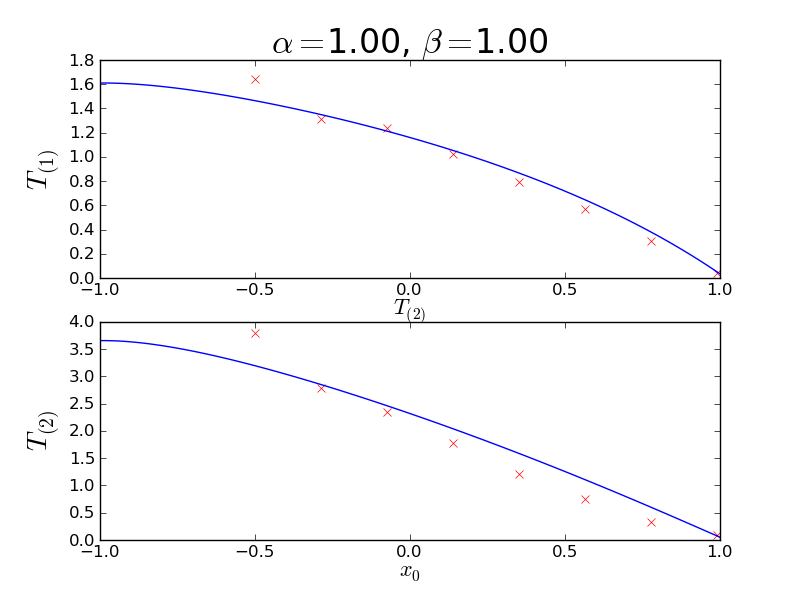
\includegraphics[width=0.48\textwidth]
{/home/alex/Workspaces/Latex/OptSpike/Figs/Moments_a=10_b=10_N=128.png}
}
\\
\subfloat[ ]
{
\label{fig:ab2}
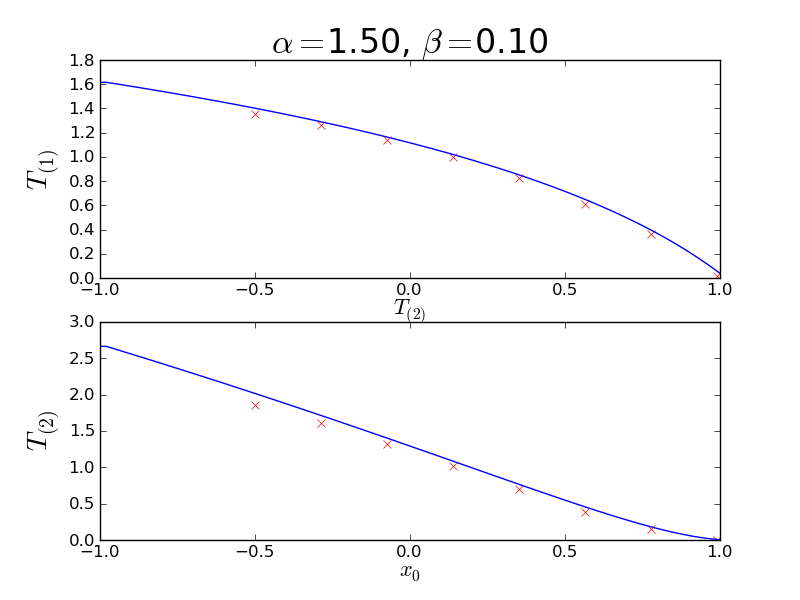
\includegraphics[width=0.48\textwidth]
{/home/alex/Workspaces/Latex/OptSpike/Figs/Moments_a=15_b=1_N=128.png}
}
\subfloat[ ]
{
\label{fig:ab2}
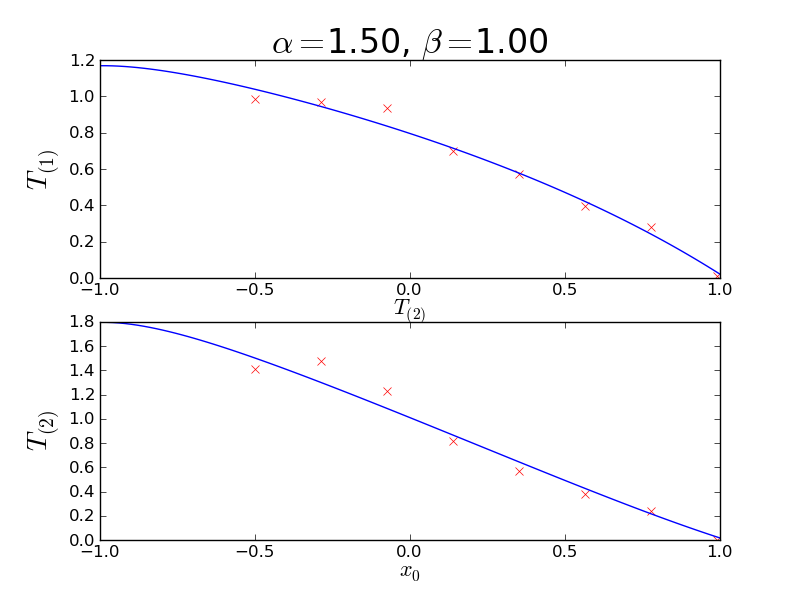
\includegraphics[width=0.48\textwidth]
{/home/alex/Workspaces/Latex/OptSpike/Figs/Moments_a=15_b=10_N=128.png}
}
\caption[]{Comparison between solutions of equations
\cref{eq:BVP_Tone,eq:BVP_Ttwo} and empirical samples from simulating
\cref{eq:X_evolution_uo} }
\label{fig:label}
\end{center}
\end{figure}





% In order to do so we must convert the problem to one starting from $.0$ Set $$ Y
% = X - x_0 $$
% 
% Then we have:
% \begin{equation}
% \begin{gathered}
% dY_s = (\atilde - \frac{Y_s}{\tc} ) \intd{s} + \b \intd{W_s},
% \\
% Y_0 = .0,
% \\
% \atilde =  \a - \tfrac{x_0}{\tc}
% \\
% \yth = \xth - x_0
% \end{gathered}
% \end{equation}
% 
% $X$ hits $\xth$ whenever $Y$ hits $\yth$ and so we use equations 15-19 in
% \cite{Ditlevsen2008a}:
% \begin{equation}
% \Exp[\t^2] = \tc^2 \left[ 
% 2\phi_1^2(\eta) -
%   \phi_2(\eta) - 
%   2\phi_1(\eta)\phi_1(\xi)+
%   \phi_2(\xi)
%   \right]
% \end{equation}
% where 
% \begin{eqnarray}
% \xi &=& \atilde\tc \sqrt{\tfrac{2}{\b^2 \tc} }
% =  \boxed{(\a - \tfrac{x_0}{\tc} ) \tc \sqrt{\tfrac{2}{\b^2 \tc}}}
% \\
% \eta &=&
% (\yth - \atilde\tc)\sqrt{\tfrac{2}{\b^2 \tc}}
% = \boxed{(\xth -\a \tc )\sqrt{\tfrac{2}{\b^2 \tc}}}
% \\
% \phi_1(z)&=&
%  \frac{1}{2} \sum_{n=1}^{\infty} \frac{(z \sqrt{2})^n}{n!}
%  \Gamma\left(\frac{n}{2}\right)
% \\
% \phi_2(z)&=& \phi_1(z) \left[ \psi\left( \tfrac{n}{2} \right) - \psi(1) \right]
% \end{eqnarray}
% where $\Gamma, \psi$ are the
% \href{http://docs.scipy.org/doc/scipy/reference/generated/scipy.special.gamma.html#scipy.special.gamma}{Gamma}
% and
% \href{http://docs.scipy.org/doc/scipy/reference/generated/scipy.special.psi.html#scipy.special.psi}{digamma}
%  functions respectively.


\bibliographystyle{plain}
\bibliography{library,local}
% \bibliography{local}

\end{document}
